\section{Delta Dictionaries}
\label{sec:DD}
Borrowing from association lists, {\dd}s use a list-of-pairs, where the first item in each list represents
a key and the second is the literal value that is mapped to the represented key. Unlike association lists,
the natural number that represents the key is not its literal value. In order to maintain canonical order,
while ensuring that every natural number is valid as the first item in a pair, that number must represent
the non-negative difference between the key it represents and the previous key. We call this a "delta",
alluding to the technique of \emph{delta encoding} which is more commonly harnessed for performance
optimization (TODO source). If the number is $0$, we get duplicate keys - to prevent this, the offset is
actually the delta plus $1$, so that a delta of $0$ indicates an offset (from the previous key) of $1$,\
whereas a delta of $2$ indicates an offset of $3$. The head of the list does not follow the "plus $1$"
rule, so the very first "delta" is interpreted literally, i.e. it represents a key of the its exact
value.

\begin{figure}[H]
  \centering
  \begin{tikzpicture}[nodes = {align = left}]
    \node [scale=.45]
    {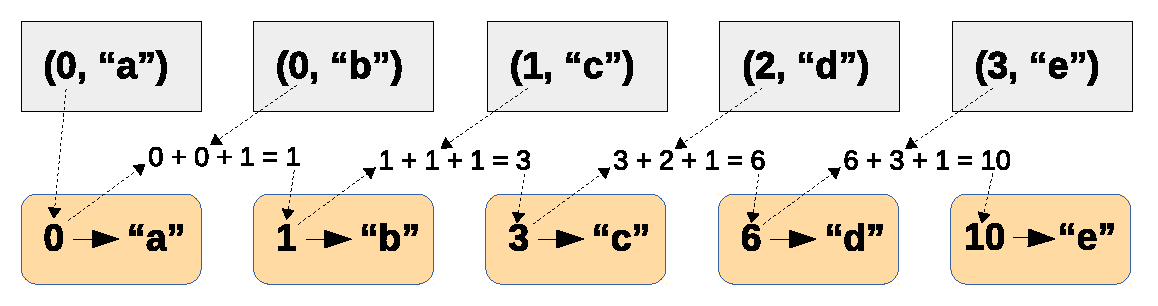
\includegraphics{figs/mech-2.eps}};
  \end{tikzpicture}
  \caption{What mapping is represented by the \dd~ $\dictP$?}
  \label{fig:mech1}
\end{figure}

\begin{figure}[H]
  \centering
  \begin{tikzpicture}[nodes = {align = left}]
    \node [scale=.4]
    {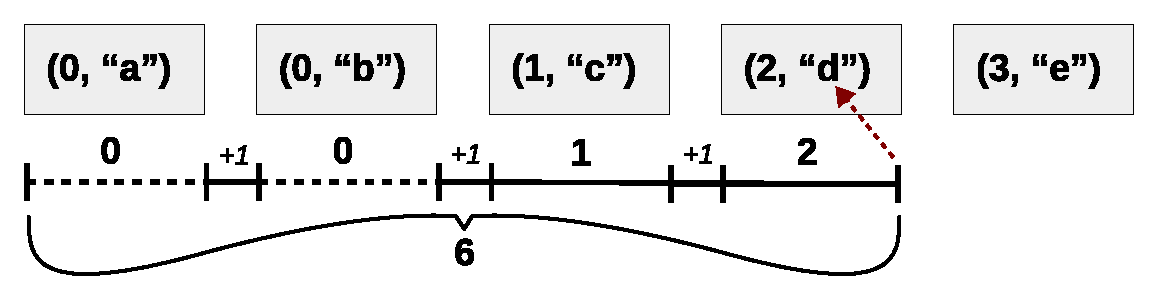
\includegraphics{figs/find-6.eps}};
  \end{tikzpicture}
  \caption{How do we find key $6$ in the \dd?}
  \label{fig:find-6}
\end{figure}

\begin{figure}[H]
  \centering
  \begin{tikzpicture}[nodes = {align = left}]
    \node [scale=.4]
    {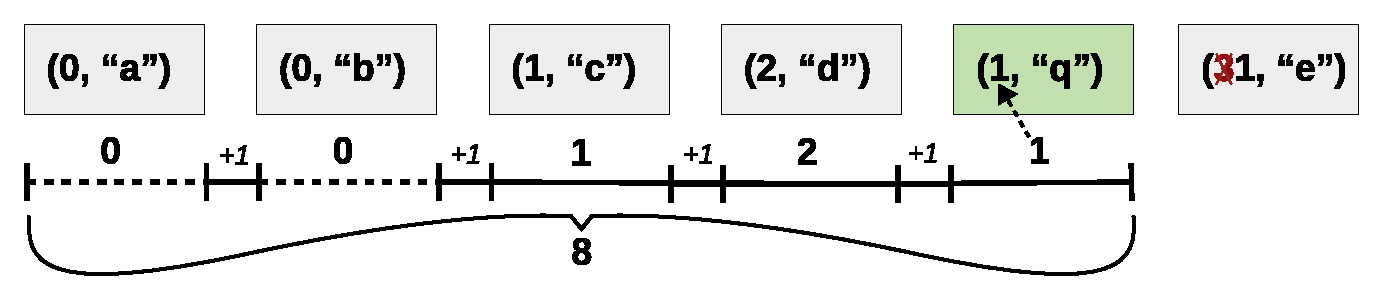
\includegraphics{figs/insert-8.eps}};
  \end{tikzpicture}
  \caption{How do we insert a mapping from key $8$ to value "q"?}
  \label{fig:find-6}
\end{figure}

In addition to the basic functionality of lookup and insertion, our Agda mechanization defines key
deletion, union, map, and to/from-list operations. It also defines and proves the core metatheory
of dictionaries (not reproduced here) as well as proofs of \SemInj, \EqDec, a destruction
theorem, and analogs to \emph{contraction} and \emph{exchange} (the theorems are reproduced below,
but the proofs are not). \SemTot~ cannot be formally defined - rather its truth is apparent from
the fact that the other theorems do not require their \dd~ arguments to be refined with
validity premises.

\begin{theorem}[\SemInj]
\label{thm:SemInj}

\breakAndIndent
%
For any {\dd}s $D_1$ and $D_2$,
%
if for all $n$, $D_1[n] = D_2[n]$,
%
then $D_1 = D_2$.

\end{theorem}

\begin{theorem}[\EqDec]
\label{thm:EqDec}

\breakAndIndent
%
For any {\dd}s $D_1$ and $D_2$ whose values are of type $A$,
%
given a function that decides equality for type $A$,
%

\justIndent
%
we can decide that either $D_1 = D_2$ or $D_1 \ne D_2$.

\end{theorem}

\begin{theorem}[\EzDstr]
\label{thm:EzDstr}

\breakAndIndent
%
For any \dd~ $D$,

\justIndent \quad
%
either $D = \emptyset$ OR

\justIndent \quad
%
there exist $D'$, $n \notin D'$, and $a$
%
s.t. $D = D' , (n, a)$.

\end{theorem}

\begin{theorem}[Dictionary Contraction]
\label{thm:cont-dicts}

\breakAndIndent
%
For any {\dd}~ $D$,
%
$D, (n, a), (n, b) = D, (n, b)$.

\end{theorem}

\begin{theorem}[Dictionary Exchange]
\label{thm:exch-dicts}

\breakAndIndent
%
For any {\dd}~ $D$,
%
if $n \ne m$, then
%
$D, (n, a), (m, b) = D, (m, b), (n, a)$.

\end{theorem}
